%%%%%%%%%%%%%%%%%%%%%%%%%%%%%%%%%%%%%%%%%%%%%%%%%%%%%%%%%%%
% PCP Cheat Sheet,
% Christian Horn <chorn@fluxcoil.net>
%
% based on:
% https://ctan.math.illinois.edu/macros/latex/contrib/tcolorbox/tcolorbox-tutorial-poster.pdf
%
%%%%%%%%%%%%%%%%%%%%%%%%%%%%%%%%%%%%%%%%%%%%%%%%%%%%%%%%%%%

\documentclass[12pt]{article}
\usepackage[a3paper,landscape]{geometry}
\usepackage{lipsum}
\usepackage{lmodern}
\usepackage{enumerate}
\usepackage{hyperref}
\usepackage{verbatim}
\usepackage[poster]{tcolorbox}
\tcbuselibrary{listings}
\pagestyle{empty}
\begin{document}

\begin{tcbposter}[
	coverage = {
		spread,
		interior style={top color=yellow,bottom color=yellow!50!red},
		watermark text={PCP cheat sheet},
		watermark color=yellow,
	},
	poster = {showframe=false,columns=4,rows=5},
	boxes = {
		enhanced standard jigsaw,sharp corners=downhill,arc=3mm,boxrule=1mm,
		colback=white,opacityback=0.75,colframe=blue,
		title style={left color=black,right color=cyan},
		fonttitle=\bfseries\Large\scshape
	}
]

% Here, we insert the poster content later

\posterbox[blankest,interior engine=path,height=3cm,
		halign=center,valign=center,fontupper=\bfseries\large,colupper=red!25!black
	]{name=title,column=1,span=3,below=top}{
	\resizebox{18cm}{!}{\bfseries\Huge Performance Co-Pilot cheat sheet}\\[3mm]
	Christian Horn \textless chorn@fluxcoil.net\textgreater
}


%----------------------------------------------------------------------------------
% Basics
%----------------------------------------------------------------------------------

\posterbox[adjusted title=PCP basics]{name=basics,
	below=title}{
	% sequence=1 between title and bottom}{

	\textbf{Installation}\\
	Package \textbf{zero-conf} pulls in dependencies, starts daemons, starts
	archiving of a default set of metrics.  On RPM based distros (RHEL,
	Fedora, CentOS etc.): \\
	    % \textit{ \hspace*{0.5cm}\# dnf -y install pcp-zeroconf \\ } \\
	    \hspace*{0.5cm}\# dnf -y install pcp-zeroconf \\
	Installation via Ansible playbook: \\
	    \hspace*{0.5cm}\# linux-system-roles.metrics \\
	Verify pcp installation: \\
	    \hspace*{0.5cm}\# pcp \\
	    \hspace*{0.5cm}\# systemctl status pmcd pmlogger \\
	
	\textbf{Important tools}\\
	Tools from package 'pcp-system-tools' can be used with either 
	the running pmcd, or PCP archive files:
	\begin{itemize}
	    \item pcp atop
	    \item pcp collectcl
	    \item pcp free
	    \item pcp iostat
	    \item pcp dstat
	\end{itemize}
	
	\textbf{Important Pathes}\\
	    \hspace*{0.5cm}/var/lib/pcp/config/ \\
	    \hspace*{0.5cm}/var/log/pcp/ \\
	    \hspace*{0.5cm}/etc/pcp/ \\
	
	\textbf{Working with metrics}\\
	Which metrics are offered by the running pmcd? \\
	    \hspace*{0.5cm}\# pminfo \\
	
	Which metrics related to cpu are available? \\
	    \hspace*{0.5cm}\# pminfo $\vert$ grep cpu \\
	
	\vspace{0.0em} % When there are two boxes, some whitespace may need to be added if the one on the right has more content
	}


%----------------------------------------------------------------------------------
% Links
%----------------------------------------------------------------------------------

\posterbox[adjusted title=Links]{name=links,column=2,span=2,above=bottom}{
	\begin{enumerate}[{[1]}]
		% \item\label{litA} Important Authors, \textit{Important Title}
    	\item \href{https://access.redhat.com/articles/1145953}{kbase: Index of  (PCP) articles, solutions, tutorials, white papers}
    	\item Ansible:\href{https://github.com/linux-system-roles/metrics}{https://github.com/linux-system-roles/metrics} \href{https://github.com/performancecopilot/ansible-pcp}{https://github.com/performancecopilot/ansible-pcp}
    	\item \href{https://pcp.io}{Performance Co-Pilot site}
		\item Articles: \href{https://www.redhat.com/en/blog/how-solve-performance-mysteries-performance-co-pilot-red-hat-enterprise-linux}{Solve performance mysteries with PCP} / \href{https://www.redhat.com/en/blog/examining-container-performance-rhel-8-pcp-and-pdma-podman}{PCP and podman} / \href{https://www.redhat.com/en/blog/implementing-dstat-performance-co-pilot}{PCP and dstat}
	\end{enumerate}
}

%----------------------------------------------------------------------------------
% Archive files
%----------------------------------------------------------------------------------

\posterbox[adjusted title=Archive files]
	{name=archivefiles,column=3,between=title and links}{
		\textbf{Basics}	\\
		Which archive is pmlogger logging into? \\
    	\hspace*{0.5cm}\# pcp \\

		Set a variable to current archive, and evaluate how many metrics
		are logged in the archive: \\
    	\hspace*{0.5cm}\# cd /var/log/pcp/pmlogger/\textless hostname\textgreater \\
    	\hspace*{0.5cm}\# pminfo -a \textless archivename\textgreater $\vert$ wc -l \\

		% TODO: more verbose syntax here
		Have pmdiff point out 'significant peaks' in archives: \\
    	\hspace*{0.5cm}\# pmdiff -a \textless archivename\textgreater \\

		\textbf{Accessing metrics} \\
		Most basic access to metrics: \\
    	\hspace*{0.5cm}\# pmstat -t 1 \\
		\hspace*{0.5cm}\# pmrep -a \textless archivename\textgreater   \textless metric\textgreater \\
    	\hspace*{0.5cm}\# pcp -a 20180831.11.31 -\/-origin @1pm \textbackslash \\
    	\hspace*{1.0cm}   dstat -\/-time -\/-disk -\/-mem 60sec 10 \\
    	\hspace*{0.5cm}\# pmrep -a 20220128 kernel.cpu -p -t 300 \textbackslash \\
    	\hspace*{1.0cm}   -\/-hostzone -S @19:30 \\
		\\
		\textbf{Graphical access} \\
    	\hspace*{0.5cm}\# pmchart \\
    	\hspace*{0.5cm}\# dnf -y install pcp2pdf; \textbackslash \\
    	\hspace*{1.0cm}   pcp2pdf -a \textless archivename\textgreater \\
}

%----------------------------------------------------------------------------------
% pmdas
%----------------------------------------------------------------------------------

\posterbox[adjusted title=pmdas]
	{name=pmdas,column=2,below=title}{
		\textbf{PMDA installation} \\
		PMDA's are code pieces capable of reading metrics from their area
		like sensors, database, and so on.
		PMDS's can be searched as packages and installed, for example on yum4/dnf
		distros: \\ 
    	\hspace*{0.5cm}\# dnf search pcp-pmda \\
    	\hspace*{0.5cm}\# dnf install -y pcp-pmda-lmsensors \\
    	\hspace*{0.5cm}\# cd /var/lib/pcp/pmdas/lmsensors \\
    	\hspace*{0.5cm}\# less README \\
    	\hspace*{0.5cm}\# ./Install
}

%----------------------------------------------------------------------------------
% pmie
%----------------------------------------------------------------------------------

\posterbox[adjusted title=pmie]
	{name=pmie,column=1,below=basics}{
		pmie, performance metrics interference engine, can react on defined
		metric states: send email on high load, and so on. \\ 
    	\hspace*{0.5cm}\# pmie -\/-verbose -\/-timestamp -\/-interval 1 \\
    	\hspace*{0.5cm}\# /etc/pcp/pmie/config.default \\
    	\hspace*{0.5cm}\# pmie -\/-archive 20200512 -\/-config \textless rules\textgreater
}

%----------------------------------------------------------------------------------
% pmdiff
%----------------------------------------------------------------------------------

\posterbox[adjusted title=Anomaly search in archives]
	{name=diff,column=2,between=pmdas and links}{
		Which metrics are remarkably different in a certain timeframe?
		Example: we had I/O problems from 2am to 3am: \\
    	\hspace*{0.5cm}\# cat cull \\
    	\hspace*{1.2cm}     rsyslog. \\
    	\hspace*{0.5cm}\# pmdiff -z -X ./cull -q 10 \textbackslash \\
    	\hspace*{1.2cm}     -\/-start @10:00 -\/-finish @10:30 \textbackslash \\
    	\hspace*{1.2cm}		-\/-begin @12:00 -\/-end @12:30 \textbackslash \\
    	\hspace*{1.2cm}		./archives/20120512 $\vert$ less \\

		What are the top 5 cpu and memory hogs? \\
    	\hspace*{0.5cm}\# pmrep proc.hog.cpu, proc.memory.rss \textbackslash \\
    	\hspace*{1.2cm}		-J 5 -1 -g -b MB \\

		What are the current PIDs, and how much rss uses process with pid 75? \\
    	\hspace*{0.5cm}\# pmrep proc.smaps.rss -g $\vert$ less \\
    	\hspace*{0.5cm}\# pmrep proc.smaps.rss -g -i '.*75.*'
}

%----------------------------------------------------------------------------------
% Remote collection
%----------------------------------------------------------------------------------

\posterbox[adjusted title=Remote collection]
	{name=remotecollection,column=4,below=top}{
		\textbf{Install PCP on clients} \\
		Setup client systems to offer metrics via pmcd: install pcp, open packet 
		based firewall, enable remote access in pmcd: \\
	\footnotesize{
	    \hspace*{0.5cm}\# yum -y install pcp \\
	    \hspace*{0.5cm}\# firewall-cmd -\/-permanent -\/-zone=public \textbackslash \\
	    \hspace*{1.1cm}   -\/-add-port=44321/tcp \\
	    \hspace*{0.5cm}\# firewall-cmd -\/-reload \\
	    \hspace*{0.5cm}\# CONFIG=/etc/sysconfig/pmcd \\
	    \hspace*{0.5cm}\# if grep -q PMCD\_LOCAL \$CONFIG; then \textbackslash \\
	    \hspace*{1.1cm}   sed -ie 's,PMCD\_LOCAL.*,PMCD\_LOCAL=0,' \textbackslash \\
	    \hspace*{1.1cm}   /etc/sysconfig/pmcd \textbackslash \\
	    \hspace*{0.9cm}   else \\
	    \hspace*{1.1cm}   echo 'PMCD\_LOCAL=0' >>/etc/sysconfig/pmcd \\
	    \hspace*{0.9cm}   fi \\
	    \hspace*{0.5cm}\# grep PMCD\_LOCAL /etc/sysconfig/pmcd \\
	    \hspace*{0.5cm}\# service pmcd restart \\
	    \hspace*{0.5cm}\# chkconfig pmcd on \\
	}

		\textbf{Install PCP on collector system} \\
	On the collector, we install pcp-zeroconf which also sets up logging to archive files.
	We then set variable CLIENT to the clients name, create a config- and controlfile,
	and notify pmlogger of the changes.
	\footnotesize{
	    \hspace*{0.5cm}\# yum -y install pcp-zeroconf \\
	    \hspace*{0.5cm}\# CLIENT=rhel7u8a \\
	    \hspace*{0.5cm}\# /usr/libexec/pcp/bin/pmlogconf \textbackslash \\
	    \hspace*{1.1cm}   /var/lib/pcp/config/pmlogger/config.\$CLIENT \\
	    \hspace*{0.5cm}\# echo "\$CLIENT.local n n " \textbackslash \\
	    \hspace*{1.1cm}   PCP\_LOG\_DIR/pmlogger/\$CLIENT.local" \textbackslash \\
	    \hspace*{1.1cm}   " -r -T30d -c config.\$CLIENT" \textbackslash \\
	    \hspace*{1.1cm}   \textgreater/etc/pcp/pmlogger/control.d/\$CLIENT \\
	    \hspace*{0.5cm}\# /usr/libexec/pcp/bin/pmlogger\_check
	}

% \includegraphics[width=10em,height=4em]{pics/s05_pcp-daemons-grafanaserver.png}
\center{
    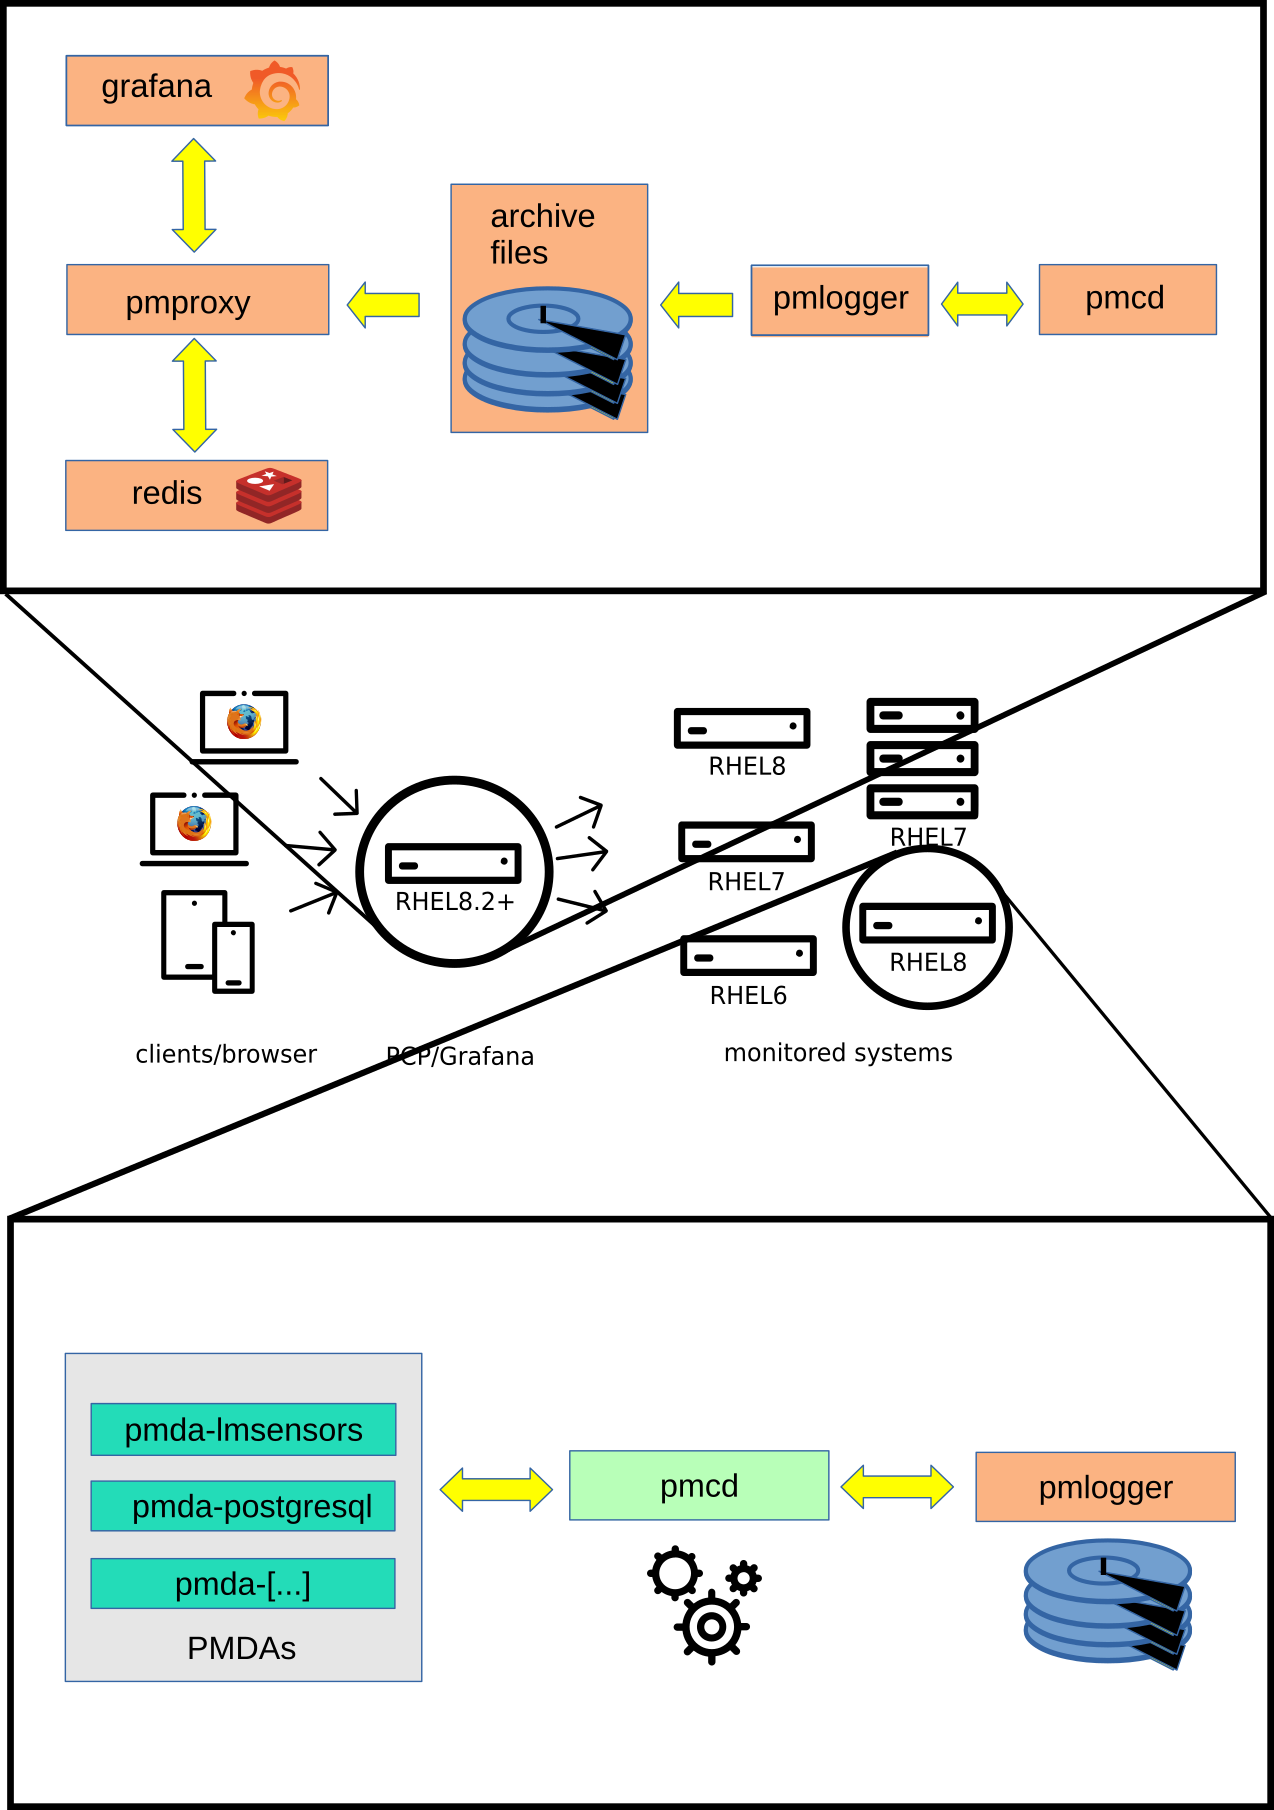
\includegraphics[width=20em]{pics/s05_browsers_pcp_servers_overview_componentsb.png}
}

% pmlogconf - configures configfile, including the pmdas you run on the system

}

\end{tcbposter}
\end{document}
